\documentclass[10pt,a4paper]{article}

% ---------- page, fonts, spacing ----------
\usepackage[a4paper,top=2.1cm,bottom=2.2cm,left=2.2cm,right=2.2cm]{geometry}
\usepackage[T1]{fontenc}
\usepackage{newtxtext,newtxmath}          % Times-style text and maths
\usepackage[final]{microtype}             % better justification, fewer over-full lines
\usepackage{setspace}
\setstretch{1.04}
\emergencystretch=1.5em
\setlength{\parindent}{1.2em}
\setlength{\parskip}{0pt}

% ---------- floats, tables, captions ----------
\usepackage{graphicx}
\usepackage{booktabs}
\usepackage{array}
\usepackage[font=small,labelfont=bf,labelsep=period,skip=4pt]{caption}
\usepackage{subcaption}
\setlength{\textfloatsep}{10pt plus 2pt minus 2pt}
\setlength{\floatsep}{8pt plus 2pt minus 2pt}
\setlength{\intextsep}{8pt plus 2pt minus 2pt}
\graphicspath{{../figures/}}
\renewcommand{\topfraction}{0.9}
\renewcommand{\bottomfraction}{0.8}
\renewcommand{\textfraction}{0.07}
\renewcommand{\floatpagefraction}{0.85}
\setcounter{topnumber}{3}
\setcounter{totalnumber}{5}

% ---------- headings ----------
\usepackage{titlesec}
\titleformat{\section}{\normalfont\large\bfseries}{\thesection}{0.6em}{}
\titleformat{\subsection}{\normalfont\normalsize\bfseries}{\thesubsection}{0.6em}{}
\titlespacing*{\section}{0pt}{10pt plus 2pt minus 2pt}{4pt}
\titlespacing*{\subsection}{0pt}{7pt plus 2pt minus 1pt}{3pt}
\titlespacing*{\paragraph}{0pt}{4pt}{0.8em}

\usepackage{amsmath}
\usepackage{xcolor}
\usepackage[hidelinks]{hyperref}
\usepackage{enumitem}
\setlist{nosep,leftmargin=1.3em}

\newcommand{\code}[1]{\texttt{\small #1}}

\begin{document}

% ---------- title block ----------
\begin{center}
{\LARGE\bfseries Classification of Countries into HDI-Based Development\\[3pt] Categories Using World Bank Indicators\par}
\vspace{8pt}
{\large DS203 Course Project, Classification Track\par}
\vspace{8pt}
{\normalsize
\begin{tabular}{ccc}
Tanish Jain & Ruturva Vaghasia & Arnav Jain\\
\small 25B4244 & \small 25B4205 & \small 25B2704
\end{tabular}\par}
\vspace{4pt}
{\small November 2026 \quad$\cdot$\quad Code and data: \url{https://github.com/tanishjain0911-beep/ds203-hdi-classification}\par}
\end{center}
\vspace{2pt}

\section{Introduction}
The Human Development Index (HDI) published by UNDP combines life expectancy, education and income into a single
score between 0 and 1. Because it depends on survey and census data, it is released with a delay of one to two
years. The World Bank, in contrast, reports economic, infrastructure and health indicators for almost every
country each year. This project asks whether such routinely available indicators are sufficient to place a country
in the correct development category, and which of them are the most informative.

We build the target from the 2023 HDI score with three classes: \textbf{Low} ($\text{HDI} < 0.550$),
\textbf{Medium/High} ($0.550 \le \text{HDI} < 0.800$) and \textbf{Very High} ($\text{HDI} \ge 0.800$). This grouping
is defined for the project and is not UNDP's official four-category classification. To avoid target leakage, we
exclude the HDI score and its components (life expectancy, expected and mean years of schooling, GNI per capita)
from the predictors and use country names and ISO codes only as identifiers. We compare four classifiers,
examine whether categorical features and PCA improve performance, and treat all results as predictive
associations, not causal effects.

\section{Methodology}
\paragraph{Data sources and matching.}
The target is the column \code{hdi\_2023} of the UNDP Human Development Report 2025 release (\emph{composite
indices complete time series}, accessed 23 November 2026). The nine predictors are World Development Indicators
downloaded as CSV files from the World Bank data portal (accessed 25 November 2026): GDP growth
(\code{NY.GDP.MKTP.KD.ZG}), inflation (\code{FP.CPI.TOTL.ZG}), unemployment (\code{SL.UEM.TOTL.ZS}), infant mortality
(\code{SP.DYN.IMRT.IN}), access to electricity (\code{EG.ELC.ACCS.ZS}), internet users (\code{IT.NET.USER.ZS}),
agriculture and industry value added (\code{NV.AGR.TOTL.ZS}, \code{NV.IND.TOTL.ZS}) and trade
(\code{NE.TRD.GNFS.ZS}), the last three as a percentage of GDP. Region is taken from the World Bank country
metadata supplied with the same download; aggregate entries (world, regional and income-group totals) have no
region and were removed. The tables were merged on ISO3 codes. All 195 UNDP countries were matched, so no manual
code corrections were required, and 22 World Bank economies without an HDI (mostly territories such as Puerto Rico
and Greenland) were excluded. Monaco and DPR Korea have no 2023 HDI and were dropped, which leaves
193 countries: 26 Low (13.5\%), 93 Medium/High (48.2\%) and 74 Very High (38.3\%).

\paragraph{Reference year and engineered feature.}
Each indicator takes its 2023 value. If that value is missing, the most recent value from 2022 or 2021 is used,
and no value later than 2023 is ever used; the year of every value is recorded in the dataset. Only 19 of the
1{,}737 predictor values come from this look-back window, and the remaining gaps are kept as missing for the
imputation experiments. \code{DominantSector} is derived from the sector shares: the services share is estimated as
$100 - \text{agriculture} - \text{industry}$, and the largest of the three shares gives the category. It is set to
missing when an input is missing or a share is negative. Services dominates in 176 countries, industry in 8 (oil and
mining economies such as Qatar, Kuwait and Libya) and agriculture in 2 (Niger and Chad); 7 values are missing.

\paragraph{Transformations.}
Inflation and trade are strongly right-skewed. Inflation has 19 values above the upper IQR fence of about 18\%,
the largest being Lebanon (221\%), Sudan (139\%) and Argentina (133\%); trade reaches 403\% of GDP in Luxembourg and
353\% in Hong Kong. These values are genuine, and no percentage variable lies outside the range 0 to 100, so no observations
were removed. Both features are instead transformed with the sign-preserving logarithm
$\operatorname{sign}(x)\ln(1+|x|)$, which is defined for the negative inflation values. The transformation has no
learned parameters, so applying it before the split does not leak information.

\paragraph{Data split and preprocessing.}
Since the observations are countries rather than a time series, we use a stratified 60/20/20 split with
\code{random\_state=42}, giving 115 training, 39 validation and 39 test countries (16, 5 and 5 of them Low). We place
all learned preprocessing in a scikit-learn \code{Pipeline} built around a \code{ColumnTransformer}, so it is
fitted on training data only and refitted within every cross-validation fold. Numerical features are imputed with
the training mean (selected in Section~\ref{sec:prep}) and standardised. Categorical features receive an explicit
``Missing'' level and are one-hot encoded with \code{handle\_unknown="ignore"}. The result is 20 model inputs.

\paragraph{Models and model selection.}
We train a majority-class baseline, multinomial logistic regression (L2 penalty, \code{max\_iter=5000}), a decision
tree and a random forest with 300 trees. Hyperparameters are selected with \code{GridSearchCV} using stratified
5-fold cross-validation on the training set and macro F1 as the criterion, so that the small Low class carries the
same weight as the other two. The search grids are $C \in \{0.01, 0.1, 1, 10, 100\}$ for logistic regression;
maximum depth $\in \{2, 3, 4, 5, \text{none}\}$ and minimum leaf size $\in \{1, 3, 5\}$ for the tree; and maximum
depth $\in \{3, 5, \text{none}\}$ and minimum leaf size $\in \{1, 3\}$ for the forest. The imputation, PCA and
feature-set experiments use the same folds with default model settings and are carried out before tuning. The
validation set is used only to compare the tuned models. Each model is then refitted on the training and
validation data (154 countries) and evaluated once on the test set; no modelling decision uses the test set.

\section{Experiments}
\subsection{Exploratory data analysis}
Missing values are unevenly distributed across features and classes (Figure~\ref{fig:missing}). Trade is missing
for 11.9\% of countries, inflation for 7.8\% and unemployment for 7.3\%, while electricity access and region are
complete. Missingness is concentrated in the least developed countries: 35\% of Low countries have at least one
missing indicator, compared with 27\% of Medium/High and 12\% of Very High countries, and a Low country has on
average 1.12 missing values against 0.22 for a Very High country. Unemployment is the only exception, with no
missing values in the Low class. The most incomplete records belong to conflict-affected countries (Eritrea, Yemen,
South Sudan, Somalia) and very small states (Tuvalu, Nauru). The data are therefore not missing completely at
random, and imputed values for Low countries are based largely on more developed countries.

\begin{figure}[!htb]
\centering
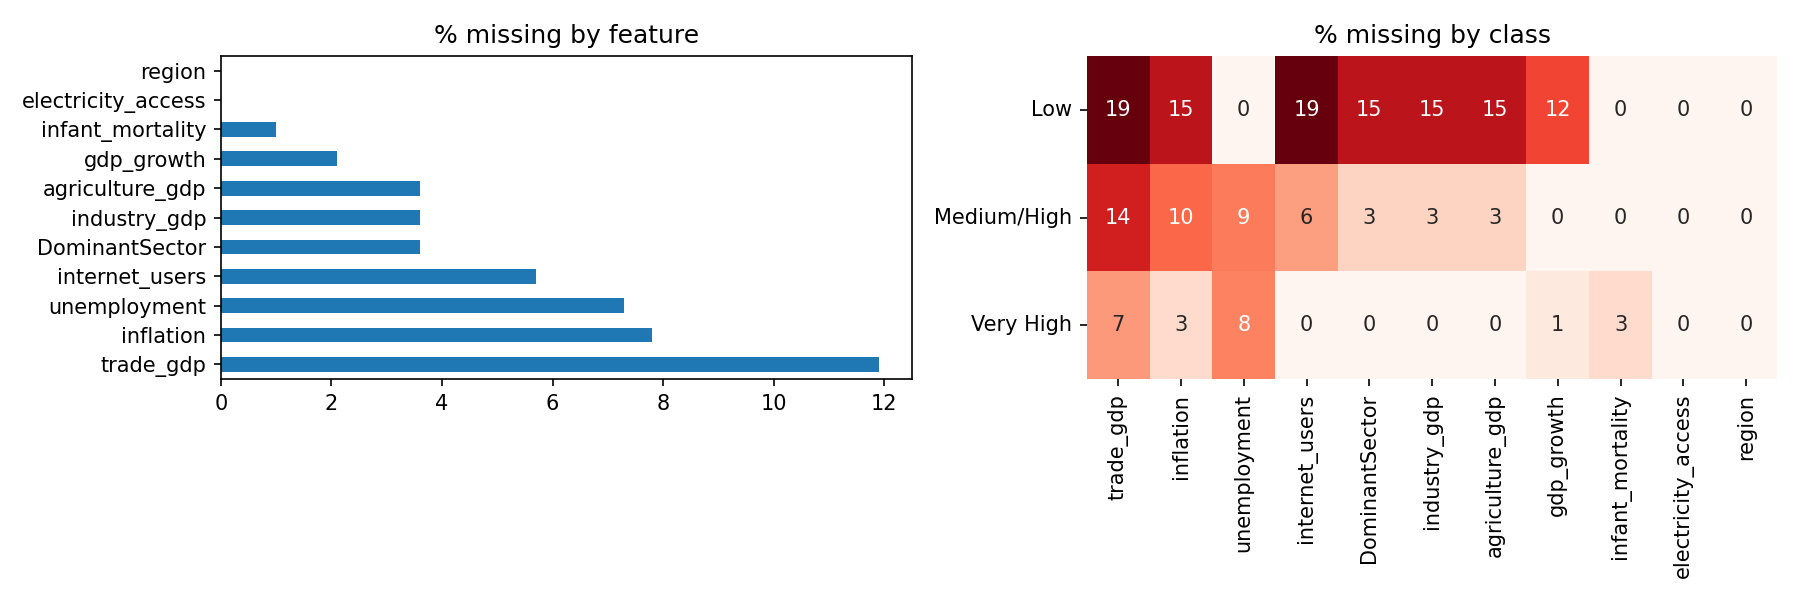
\includegraphics[width=0.86\textwidth]{missingness.png}
\caption{Share of missing values by feature (left) and by HDI class (right), in percent.}
\label{fig:missing}
\end{figure}

The health and infrastructure indicators separate the classes most clearly. From Low to Medium/High to Very High,
the median infant mortality rate falls from 45.7 to 17.7 to 4.0 per 1{,}000 live births, internet use rises from
24\% to 70\% to 92\%, electricity access from 45\% to 99\% to 100\%, and the agriculture share of GDP falls from 29\%
to 10\% to 2\%. Trade is higher in Very High countries (median 107\% of GDP against 55\% for Low), GDP growth is
slightly higher in Low countries (4.3\% against 2.0\%), and unemployment and the industry share show no consistent
ordering. Six pairs of predictors have $|r| \ge 0.5$, all within the same group of four indicators: electricity and
internet ($r = 0.84$), infant mortality and internet ($-0.83$), internet and agriculture ($-0.81$), infant mortality
and electricity ($-0.79$), infant mortality and agriculture ($0.72$), and electricity and agriculture ($-0.66$).
These indicators largely measure a common level of development. Region is also strongly associated with the
class: 22 of the 26 Low countries are in Sub-Saharan Africa and the remaining 4 in the Middle East \& North Africa,
44 of the 51 countries in Europe \& Central Asia are Very High, and all six South Asian countries are Medium/High.

\subsection{Preprocessing choices and PCA}\label{sec:prep}
Mean imputation without missingness indicators gave the highest
cross-validated macro F1 for both logistic regression ($0.839 \pm 0.068$) and the random forest ($0.890 \pm 0.061$),
compared with 0.818 and 0.875 for median imputation. A missingness indicator is a binary column marking an imputed
value, which allows a model to use the fact that a value was not reported. Given the pattern above, this signal is
plausible, but adding the indicators reduced macro F1 to 0.797 and 0.881, most likely because the additional,
mostly zero columns add noise with only 115 training countries. All differences were within one standard
deviation, and we use mean imputation without indicators.

We fitted PCA to the preprocessed training features (Figure~\ref{fig:pca}). The first component explains 38.8\% of
the variance, and seven of the 20 components are required to reach 90\%. PC1 is a development axis, with loadings
on internet use ($+0.48$), electricity access ($+0.46$), infant mortality ($-0.46$) and agriculture share ($-0.45$),
while PC2 mainly reflects short-run macroeconomic conditions (GDP growth $+0.69$, inflation $-0.41$). Along PC1 the
Low class is clearly separated, whereas Medium/High and Very High overlap. Retaining two or three components
increased the cross-validated macro F1 of logistic regression to 0.857, which is within one standard deviation of
the model without PCA, whereas every PCA setting reduced the random forest's score (0.82 to 0.87 against 0.890),
because tree splits on individual original features are more informative than splits on rotated components. The
final models therefore do not use PCA, which also keeps them interpretable in terms of the original indicators.

\begin{figure}[!htb]
\centering
\begin{subfigure}[b]{0.50\textwidth}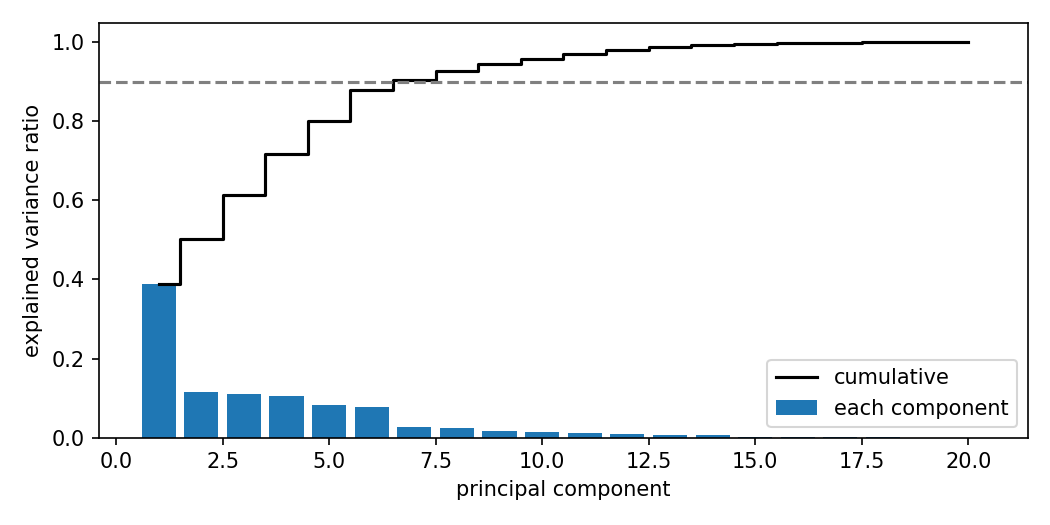
\includegraphics[width=\linewidth]{pca_explained_variance.png}\end{subfigure}\hfill
\begin{subfigure}[b]{0.42\textwidth}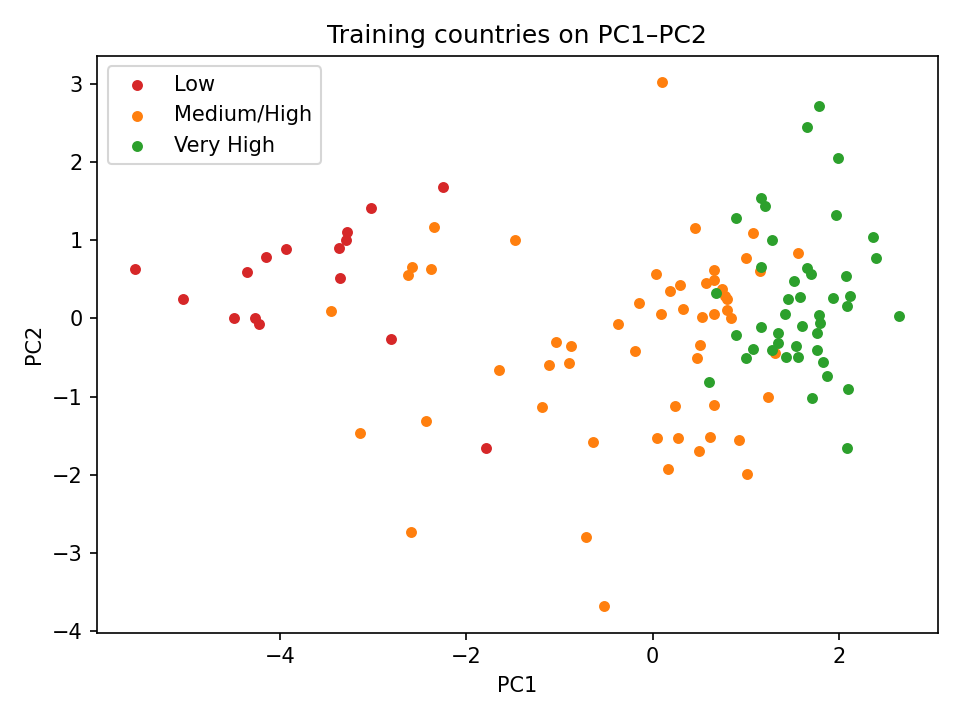
\includegraphics[width=\linewidth]{pca_scatter.png}\end{subfigure}
\caption{PCA of the preprocessed training features. Left: explained variance ratio per component and cumulative
total. Right: training countries projected onto the first two components.}
\label{fig:pca}
\end{figure}

\begin{table}[!htb]
\centering\small
\begin{tabular}{lcc}
\toprule
Feature set & Logistic regression & Random forest\\
\midrule
Numerical only & 0.846 & 0.888\\
Categorical only (region and sector) & 0.512 & 0.545\\
Numerical and region & 0.837 & 0.890\\
Numerical and \code{DominantSector} & 0.846 & 0.895\\
Combined (all features) & 0.839 & 0.890\\
\bottomrule
\end{tabular}
\caption{Cross-validated macro F1 for different feature sets (training set, five folds).}
\label{tab:features}
\end{table}

The numerical indicators carry almost all of the signal (Table~\ref{tab:features}). The categorical
features alone reach a macro F1 of about 0.5, mainly because region identifies Sub-Saharan Africa. Adding region
or \code{DominantSector} to the numerical features changes macro F1 by at most 0.01, so neither improves prediction
in a meaningful way. For the sector this is expected, since it is almost always ``Services'' and is derived from
shares that are already included. We retain the combined feature set, as the differences are within $\pm 0.01$
and it allows the role of region to be discussed.

\subsection{Model selection}
All three models clearly outperform the baseline (Table~\ref{tab:cv}). The random forest has the highest
cross-validated macro F1, but its margin over logistic regression (0.046) is smaller than the standard deviation
across folds, and logistic regression is slightly ahead on the validation set. With about 23 countries per fold,
of which only three or four are Low, the ranking of these two models is not reliable. Logistic regression selects
$C = 100$, the weakest regularisation in the grid, and is therefore close to an unregularised multinomial model.

\begin{table}[!htb]
\centering\small
\begin{tabular}{lccl}
\toprule
Model & CV macro F1 & Validation macro F1 & Selected hyperparameters\\
\midrule
Majority baseline & $0.216 \pm 0.000$ & 0.218 & predicts Medium/High\\
Logistic regression & $0.849 \pm 0.094$ & 0.799 & $C = 100$\\
Decision tree & $0.801 \pm 0.071$ & 0.703 & max.\ depth 4, min.\ leaf 3\\
Random forest & $0.895 \pm 0.074$ & 0.784 & max.\ depth 5, min.\ leaf 1\\
\bottomrule
\end{tabular}
\caption{Cross-validated macro F1 on the training set (mean $\pm$ standard deviation over five folds) and macro F1
on the validation set, using all features.}
\label{tab:cv}
\end{table}

\subsection{Test-set evaluation}
On the test set, logistic regression achieves the highest macro F1 and balanced accuracy (both 0.708), while the
random forest has the highest accuracy (0.821) and an almost perfect Very High class (F1 0.97), as shown in
Table~\ref{tab:test}. The Low class is the main weakness: logistic regression identifies two of the five Low test
countries, the random forest one and the decision tree none. As a single country changes accuracy by 2.6
percentage points, the test ranking is sensitive to individual countries, and all test scores are below the
cross-validation estimates.

\begin{table}[!htb]
\centering\small
\begin{tabular}{lcccccc}
\toprule
 & & Balanced & Macro & \multicolumn{3}{c}{F1 by class}\\
\cmidrule(lr){5-7}
Model & Accuracy & accuracy & F1 & Low & Medium/High & Very High\\
\midrule
Majority baseline & 0.487 & 0.333 & 0.218 & 0.00 & 0.66 & 0.00\\
Logistic regression & 0.795 & \textbf{0.708} & \textbf{0.708} & 0.40 & 0.79 & 0.93\\
Decision tree & 0.667 & 0.512 & 0.497 & 0.00 & 0.72 & 0.77\\
Random forest & \textbf{0.821} & 0.676 & 0.682 & 0.25 & 0.83 & 0.97\\
\bottomrule
\end{tabular}
\caption{Results on the 39 held-out test countries (5 Low, 19 Medium/High, 15 Very High).}
\label{tab:test}
\end{table}

\begin{figure}[!htb]
\centering
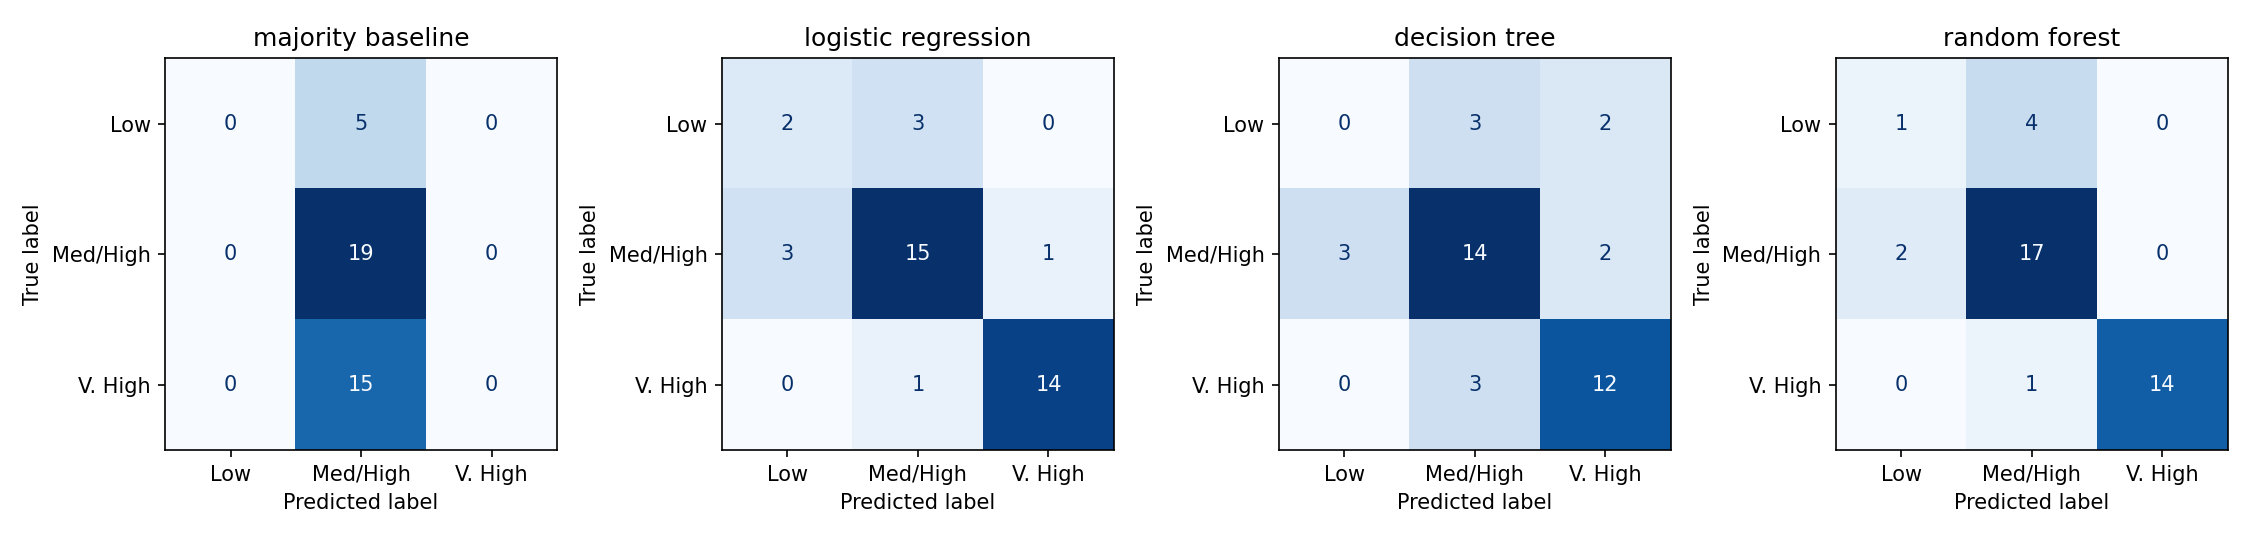
\includegraphics[width=\textwidth]{confusion_matrices.png}
\caption{Confusion matrices on the test set (rows: true class; columns: predicted class).}
\label{fig:cm}
\end{figure}

Almost all errors occur between neighbouring classes (Figure~\ref{fig:cm}). Logistic regression and the random
forest never confuse Low with Very High; only the decision tree assigns two Low countries to Very High. Six of the
random forest's seven errors involve countries with an HDI between 0.503 and 0.582, close to the 0.550 threshold:
Eritrea, Sudan, Djibouti and Gambia are Low but are predicted Medium/High, while Tanzania (0.555) and Uganda (0.582)
are predicted Low. The only misclassified Very High country is Saint Kitts and Nevis (0.840). Countries this close
to a threshold have indicator profiles similar to the neighbouring class, so these errors come from the hard cut-off as much
as from the model.

\subsection{Feature importance and interpretation}
We compute permutation importance for the random forest out of fold on the training and validation data, since
the test set contains only five Low countries. Electricity access is the most important feature (macro F1 drops by
0.171 when it is permuted), followed by infant mortality (0.096), internet use (0.073) and the agriculture share
(0.048). Region contributes 0.026, and \code{DominantSector}, unemployment, industry share, GDP growth, inflation and
trade contribute 0.010 or less. The logistic regression coefficients, which refer to standardised features, show
the same pattern: higher infant mortality raises the score of the Low class ($+3.01$) and strongly lowers that of
the Very High class ($-5.28$), the agriculture share behaves similarly, and internet use raises the Very High score
($+3.61$). Because these predictors are highly correlated and the model is almost unregularised, the division of
weight among them is unstable, and individual coefficients should not be read as separate effects. Correlation
also lowers permutation importance, since the forest can partly rely on a correlated feature when one is permuted.

\paragraph{Limitations.}
Only 26 countries are Low and 5 of them are in the test set, so a single country changes Low-class recall by
20 percentage points; for this reason we use stratified splits, macro F1 and balanced accuracy, and class
weighting is left for future work. With 193 countries, the cross-validation standard deviations (0.07 to 0.09) are as
large as the differences between models. Missing data are concentrated in the poorest countries, where mean
imputation moves values towards the sample average and may blur the Low class. Nineteen feature values come from
2021 or 2022 while the HDI refers to 2023, and annual indicators such as Sudan's GDP growth of $-29\%$ reflect
short-run shocks rather than long-run development. Finally, the results are associations: electricity access and
low infant mortality predict a high HDI, but both are also outcomes of development and are correlated with the
excluded income and education components, so changing one indicator would not necessarily change a country's class.

\paragraph{Conclusion.}
Four health and infrastructure indicators (electricity access, infant mortality, internet use and the agriculture
share of GDP) are sufficient to place most countries in the correct category. Logistic regression and the random
forest reach 79\% and 82\% test accuracy against 49\% for the majority baseline, with cross-validated macro F1 between
0.85 and 0.90. Region, the engineered sector feature and PCA add little to these indicators. The Low class remains
the most difficult, because it is small, has the most missing data and contains many countries close to the
threshold.

\end{document}
